\documentclass[a4paper,12pt,twoside]{memoir}

% Castellano
\usepackage[spanish,es-tabla]{babel}
\selectlanguage{spanish}
\usepackage[utf8]{inputenc}
\usepackage[T1]{fontenc}
\usepackage{lmodern} % scalable font
\usepackage{microtype}
\usepackage{placeins}

\RequirePackage{booktabs}
\RequirePackage[table]{xcolor}
\RequirePackage{xtab}
\RequirePackage{multirow}

% Links
\PassOptionsToPackage{hyphens}{url}\usepackage[colorlinks]{hyperref}
\hypersetup{
	allcolors = {red}
}

% Ecuaciones
\usepackage{amsmath}

% Rutas de fichero / paquete
\newcommand{\ruta}[1]{{\sffamily #1}}

% Párrafos
\nonzeroparskip

% Huérfanas y viudas
\widowpenalty100000
\clubpenalty100000

% Evitar solapes en el header
\nouppercaseheads

% Imagenes
\usepackage{graphicx}
\newcommand{\imagen}[2]{
	\begin{figure}[!h]
		\centering
		\includegraphics[width=0.9\textwidth]{#1}
		\caption{#2}\label{fig:#1}
	\end{figure}
	\FloatBarrier
}

\newcommand{\imagenflotante}[2]{
	\begin{figure}%[!h]
		\centering
		\includegraphics[width=0.9\textwidth]{#1}
		\caption{#2}\label{fig:#1}
	\end{figure}
}



% El comando \figura nos permite insertar figuras comodamente, y utilizando
% siempre el mismo formato. Los parametros son:
% 1 -> Porcentaje del ancho de página que ocupará la figura (de 0 a 1)
% 2 --> Fichero de la imagen
% 3 --> Texto a pie de imagen
% 4 --> Etiqueta (label) para referencias
% 5 --> Opciones que queramos pasarle al \includegraphics
% 6 --> Opciones de posicionamiento a pasarle a \begin{figure}
\newcommand{\figuraConPosicion}[6]{%
  \setlength{\anchoFloat}{#1\textwidth}%
  \addtolength{\anchoFloat}{-4\fboxsep}%
  \setlength{\anchoFigura}{\anchoFloat}%
  \begin{figure}[#6]
    \begin{center}%
      \Ovalbox{%
        \begin{minipage}{\anchoFloat}%
          \begin{center}%
            \includegraphics[width=\anchoFigura,#5]{#2}%
            \caption{#3}%
            \label{#4}%
          \end{center}%
        \end{minipage}
      }%
    \end{center}%
  \end{figure}%
}

%
% Comando para incluir imágenes en formato apaisado (sin marco).
\newcommand{\figuraApaisadaSinMarco}[5]{%
  \begin{figure}%
    \begin{center}%
    \includegraphics[angle=90,height=#1\textheight,#5]{#2}%
    \caption{#3}%
    \label{#4}%
    \end{center}%
  \end{figure}%
}
% Para las tablas
\newcommand{\otoprule}{\midrule [\heavyrulewidth]}
%
% Nuevo comando para tablas pequeñas (menos de una página).
\newcommand{\tablaSmall}[5]{%
 \begin{table}
  \begin{center}
   \rowcolors {2}{gray!35}{}
   \begin{tabular}{#2}
    \toprule
    #4
    \otoprule
    #5
    \bottomrule
   \end{tabular}
   \caption{#1}
   \label{tabla:#3}
  \end{center}
 \end{table}
}

%
%Para el float H de tablaSmallSinColores
\usepackage{float}

%
% Nuevo comando para tablas pequeñas (menos de una página).
\newcommand{\tablaSmallSinColores}[5]{%
 \begin{table}[H]
  \begin{center}
   \begin{tabular}{#2}
    \toprule
    #4
    \otoprule
    #5
    \bottomrule
   \end{tabular}
   \caption{#1}
   \label{tabla:#3}
  \end{center}
 \end{table}
}

\newcommand{\tablaApaisadaSmall}[5]{%
\begin{landscape}
  \begin{table}
   \begin{center}
    \rowcolors {2}{gray!35}{}
    \begin{tabular}{#2}
     \toprule
     #4
     \otoprule
     #5
     \bottomrule
    \end{tabular}
    \caption{#1}
    \label{tabla:#3}
   \end{center}
  \end{table}
\end{landscape}
}

%
% Nuevo comando para tablas grandes con cabecera y filas alternas coloreadas en gris.
\newcommand{\tabla}[6]{%
  \begin{center}
    \tablefirsthead{
      \toprule
      #5
      \otoprule
    }
    \tablehead{
      \multicolumn{#3}{l}{\small\sl continúa desde la página anterior}\\
      \toprule
      #5
      \otoprule
    }
    \tabletail{
      \hline
      \multicolumn{#3}{r}{\small\sl continúa en la página siguiente}\\
    }
    \tablelasttail{
      \hline
    }
    \bottomcaption{#1}
    \rowcolors {2}{gray!35}{}
    \begin{xtabular}{#2}
      #6
      \bottomrule
    \end{xtabular}
    \label{tabla:#4}
  \end{center}
}

%
% Nuevo comando para tablas grandes con cabecera.
\newcommand{\tablaSinColores}[6]{%
  \begin{center}
    \tablefirsthead{
      \toprule
      #5
      \otoprule
    }
    \tablehead{
      \multicolumn{#3}{l}{\small\sl continúa desde la página anterior}\\
      \toprule
      #5
      \otoprule
    }
    \tabletail{
      \hline
      \multicolumn{#3}{r}{\small\sl continúa en la página siguiente}\\
    }
    \tablelasttail{
      \hline
    }
    \bottomcaption{#1}
    \begin{xtabular}{#2}
      #6
      \bottomrule
    \end{xtabular}
    \label{tabla:#4}
  \end{center}
}

%
% Nuevo comando para tablas grandes sin cabecera.
\newcommand{\tablaSinCabecera}[5]{%
  \begin{center}
    \tablefirsthead{
      \toprule
    }
    \tablehead{
      \multicolumn{#3}{l}{\small\sl continúa desde la página anterior}\\
      \hline
    }
    \tabletail{
      \hline
      \multicolumn{#3}{r}{\small\sl continúa en la página siguiente}\\
    }
    \tablelasttail{
      \hline
    }
    \bottomcaption{#1}
  \begin{xtabular}{#2}
    #5
   \bottomrule
  \end{xtabular}
  \label{tabla:#4}
  \end{center}
}



\definecolor{cgoLight}{HTML}{EEEEEE}
\definecolor{cgoExtralight}{HTML}{FFFFFF}

%
% Nuevo comando para tablas grandes sin cabecera.
\newcommand{\tablaSinCabeceraConBandas}[5]{%
  \begin{center}
    \tablefirsthead{
      \toprule
    }
    \tablehead{
      \multicolumn{#3}{l}{\small\sl continúa desde la página anterior}\\
      \hline
    }
    \tabletail{
      \hline
      \multicolumn{#3}{r}{\small\sl continúa en la página siguiente}\\
    }
    \tablelasttail{
      \hline
    }
    \bottomcaption{#1}
    \rowcolors[]{1}{cgoExtralight}{cgoLight}

  \begin{xtabular}{#2}
    #5
   \bottomrule
  \end{xtabular}
  \label{tabla:#4}
  \end{center}
}




\graphicspath{ {./img/} }

% Capítulos
\chapterstyle{bianchi}
\newcommand{\capitulo}[2]{
	\setcounter{chapter}{#1}
	\setcounter{section}{0}
	\setcounter{figure}{0}
	\setcounter{table}{0}
	\chapter*{#2}
	\addcontentsline{toc}{chapter}{#2}
	\markboth{#2}{#2}
}

% Apéndices
\renewcommand{\appendixname}{Apéndice}
\renewcommand*\cftappendixname{\appendixname}

\newcommand{\apendice}[1]{
	%\renewcommand{\thechapter}{A}
	\chapter{#1}
}

\renewcommand*\cftappendixname{\appendixname\ }

% Formato de portada
\makeatletter
\usepackage{xcolor}
\newcommand{\tutor}[1]{\def\@tutor{#1}}
\newcommand{\course}[1]{\def\@course{#1}}
\definecolor{cpardoBox}{HTML}{E6E6FF}
\def\maketitle{
  \null
  \thispagestyle{empty}
  % Cabecera ----------------
\noindent
\includegraphics[width=\textwidth]{cabecera}\vspace{1cm}%
  \vfill
  % Título proyecto y escudo informática ----------------
  \colorbox{cpardoBox}{%
    \begin{minipage}{.8\textwidth}
      \vspace{.5cm}\Large
      \begin{center}
      \textbf{TFG del Grado en Ingeniería Informática}\vspace{.6cm}\\
      \textbf{\LARGE\@title{}}
      \end{center}
      \vspace{.2cm}
    \end{minipage}

  }%
  \hfill\begin{minipage}{.20\textwidth}
    
\includegraphics[width=\textwidth]{escudoInfor}
  \end{minipage}
  \vfill
  % Datos de alumno, curso y tutores ------------------
  \begin{center}%
  {%
    \noindent\LARGE
    Presentado por \@author{}\\ 
    en Universidad de Burgos --- \@date{}\\
    Tutor académico: \@tutor{}\\
    Tutor empresarial (ITCL): Alejandro Langarica Aparicio
  }%
  \end{center}%
  \null
  \cleardoublepage
  }
\makeatother


% Datos de portada
\title{Control Robótico mediante Tecnologías Inmersivas \\Documentación Técnica}
\author{Víctor de la Iglesia García}
\tutor{Carlos Cambra Baseca}
\date{\today}

\begin{document}
\maketitle



\cleardoublepage



%%%%%%%%%%%%%%%%%%%%%%%%%%%%%%%%%%%%%%%%%%%%%%%%%%%%%%%%%%%%%%%%%%%%%%%%%%%%%%%%%%%%%%%%



\frontmatter


\clearpage

% Indices
\tableofcontents

\clearpage

\listoffigures

\clearpage

\listoftables

\clearpage

\mainmatter

\appendix

\apendice{Plan de Proyecto Software}

\section{Introducción}
El plan de proyecto software relaciona todo aquello referido a la gestión del proyecto. Es un proceso muy importante para realizar antes de comenzar a trabajar en el desarrollo. En este punto, se llevan a cabo cosas como la planificación de tiempos para realizar las tareas, se definen los costes económicos del proyecto o l,a forma de trabajo.

Veremos dentro de la planificación temporal la manera en la que el trabajo y sus cargas han sido repartidas a lo largo de este tiempo desarrollando el proyecto. Todo esto tras haber analizado tanto el número de tareas a realizar, como la naturaleza de todas estas. 

Por otra parte, a través del estudio de viabilidad podremos poner la vista en las partes ecnómicas del proyecto. Analizaremos los costes derivados del proyecto y la gestión de las licencias utilizadas.

Podremos encontrar dos partes diferenciadas dentro de ese apartado:
\begin{itemize}
    \item Estudio de la viabilidad económica: Costes del proyecto dividiendo y analizando tanto en hardware, software como en personal.
    \item Estudio de la viabilidad legal: Análisis de las licencias para el uso de software especializado en el proyecto.
\end{itemize}

\section{Planificación temporal}
Como se comenta dentro de la memoria de este proyecto, la manera de trabajar y la metodología utilizada es la de SCRUM\cite{SCRUM} dentro del marco de las metodologías ágiles de desarrollo de software. Planificando dividiendo el tiempo en sprints que han de cubrirse en el tiempo marcado, con revisiones periódicas del trabajo.

Dentro de esto podemos ver que las 300 horas asignadas desde la Universidad de Burgos e ITCL\cite{itcl} han sido divididas en un total de seis sprints, cuya duración son de un total de dos semanas en todos los casos. 

Además, comentar que podríamos considerar como un sprint previo al trabajo la primera semana donde se realizó la toma de decisiones en referencia a lo que se iba a hacer, planificación de tareas y la metodología a seguir en cuanto a la forma de trabajar. También vimos que repositorios utilizaríamos, herramientas para la gestión o el control de versiones.  
\subsection{\textbf{Sprint 1 (07/03/2022-18/03/2022)}}
En este primer sprint se llevaron a cabo las instalaciones de aquellos softwares necesarios para el correcto desarrollo de esta parte del trabajo. También se establecieron unos puntos a cumplir relacionados en primer lugar con el 'aterrizaje' en el proyecto y en segundo lugar con el aprendizaje relativo a los guantes hápticos Nova \cite{SGloveNova}.

Las tareas dispuestas a cumplir son:
\begin{itemize}
    \item Continuar con el estudio de algunos aspectos de Unity\cite{Unity}.
    \item Estudio documentación relativa a los guantes y su SDK.
    \item Monitorizar y parametrizar lo que ofrecen los guantes.
    \item Desarrollo script que recoja datos de los guantes y aplique fuerzas hápticas\cite{Haptica1} o vibraciones.
    \item Desarrollo escena de representación 3D con \begin{enumerate}
        \item Paneles que controlen las fuerzas y vibraciones.
        \item Paneles que muestren datos de los sensores.
    \end{enumerate}
\end{itemize}

El desarrollo de este primer sprint se saldó de manera correcta sirviendo así para poder adaptarme fácilmente al proyecto y la empresa.


\newpage
\begin{figure}[t]
\centering
\label{Cierre de tareas del SPRINT 1}
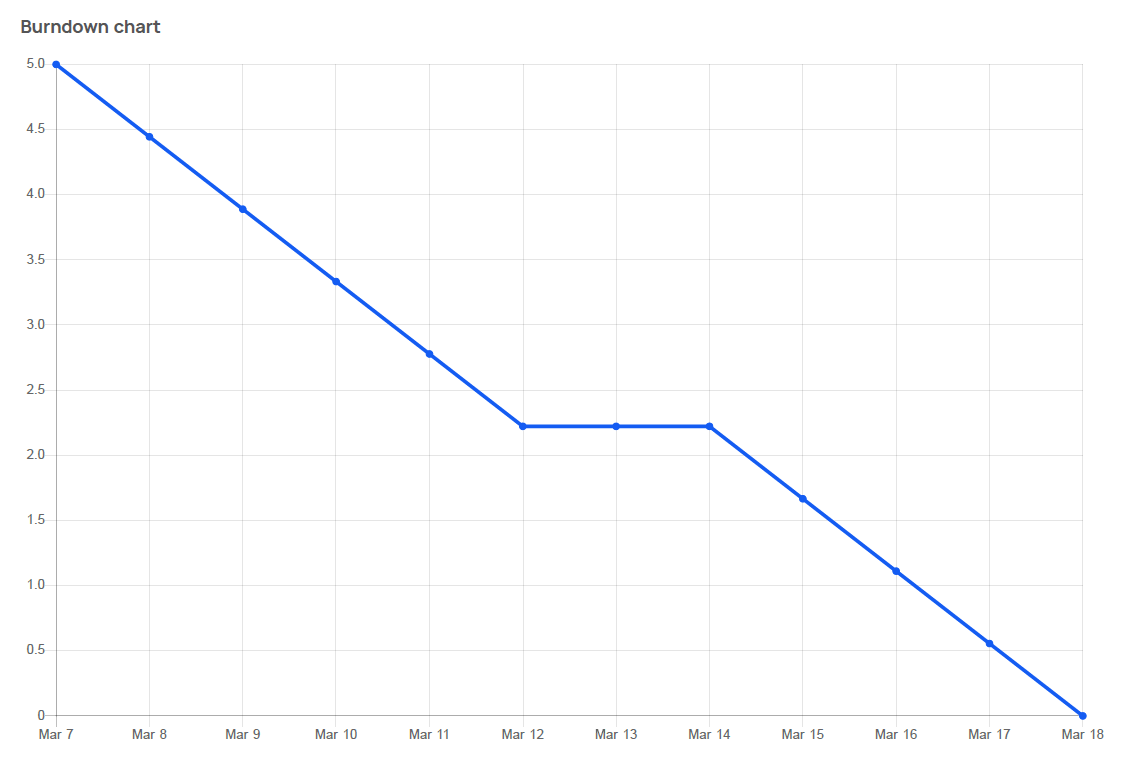
\includegraphics[width=0.6\textwidth]{img/sprint1.PNG}
\caption{Cierre de tareas del SPRINT 1}
\end{figure}

\subsection{\textbf{Sprint 2 (21/03/2022-01/04/2022)}}
En este segundo sprint los objetivos iban encaminados a mezclar por primera vez tanto el dispositivo Oculus Quest 2\cite{Quest2} y los guantes Nova. Se llevó a cabo la instalación del software de Oculus y llevamos a cabo la primera conexión. Se realizaron pruebas con ellas.

Para dar por correcta esta fusión de ambas partes teníamos las siguientes tareas:
\begin{itemize}
    \item Estudio de la componente\cite{Componentes} Transform de Unity, enfatizando en la posición.
    \item Análisis de las posibilidades de seguimiento (tracking) de Oculus.
    \item Sincronización de la vista en el mundo virtual con la visión de las gafas.
    \item Crear una escena con la adaptación de la primera escena a la realidad virtual.
    \item Cambiar el panel de fuerzas por uno que muestre datos de seguimiento.
    \item Representación tridimensional de la mano con desplazamiento en el espacio.
\end{itemize}
Para llevar a cabo estas tareas surgieron otras como que hizo falta repasar algunos conceptos de Unity, así como desarrollar scripts que funcionaran como conectores entre tecnologías para representar correctamente en el espacio las manos. También derivado de estas tareas fue el montaje del soporte de Oculus para los guantes.

\begin{figure}[h]
\centering
\label{Cierre de tareas del SPRINT 2}
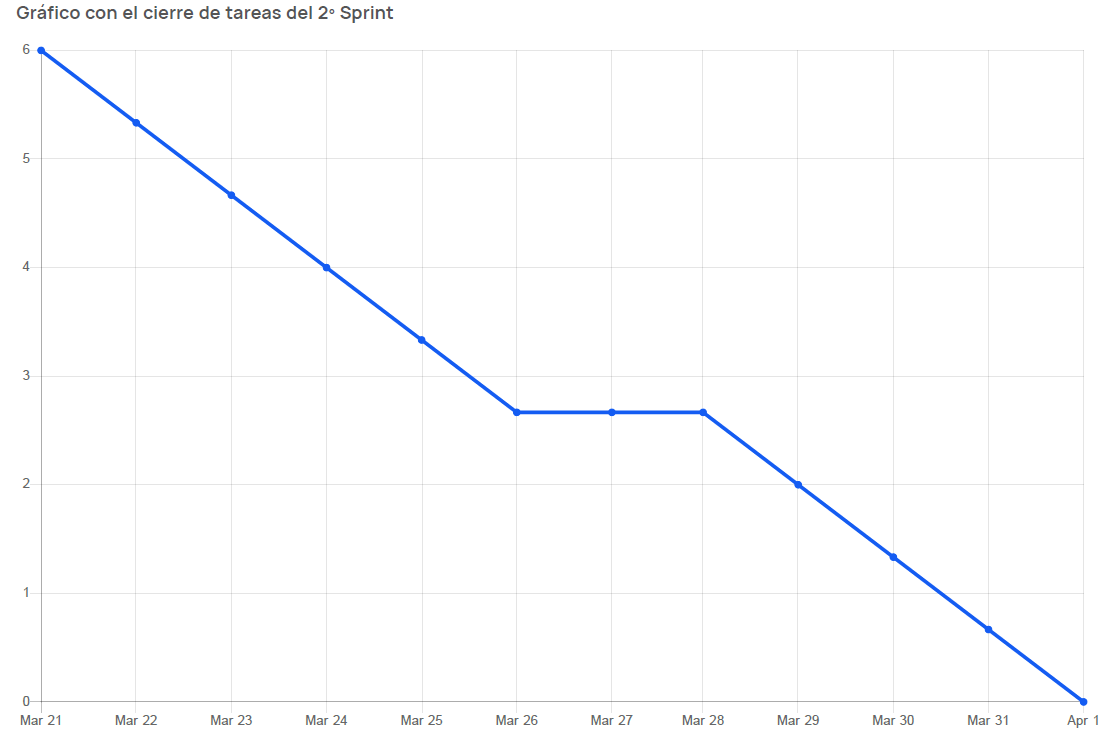
\includegraphics[width=0.6\textwidth]{img/sprint2.PNG}
\caption{Cierre de tareas del SPRINT 2}
\end{figure}
\subsection{\textbf{Sprint 3 (04/04/2022-15/04/2022)}}
Una vez llevada a cabo la conexión de ambas tecnologías, el objetivo era buscar poco a poco la manera de trabajar con el robot a nivel virtual. Para ello, intentaríamos crear un robot virtual a partir de un modelo diseñado que se comporte de maneras similares. 

Las tareas dispuestas para este sprint fueron:
\begin{itemize}
    \item Estudio de la componente\cite{Componentes} Transform de Unity, enfatizando en la rotación y sus valores.
    \item Creación de nueva escena para la replicación virtual de la pinza del robot.
    \item Implementación de métodos: \begin{enumerate}
        \item Get y Set de la posción en el espacio tridimensional.
        \item Get y Set de la apertura de la pinza.
        \item Movimiento en el espacio dada una velocidad lineal y una posición objetivo.
        \item Movimiento que controla la apertura de pinza dada una velocidad de apertura y una apertura objetivo.
    \end{enumerate}
    \item Unificar rotación de cada brazo de la pinza para abrir y cerrar de manera correcta.
    \item Ejecución de pruebas para comprobar el funcionamiento.
\end{itemize}

En este sprint he visto clave el tener que conocer a fondo la manera en la que funcionan las rotaciones dentro de este motor gráfico, ya que tuve alguna complicación a la hora de gestionar estos aspectos en el proyecto.
\begin{figure}[h]
\centering
\label{Cierre de tareas del SPRINT 3}
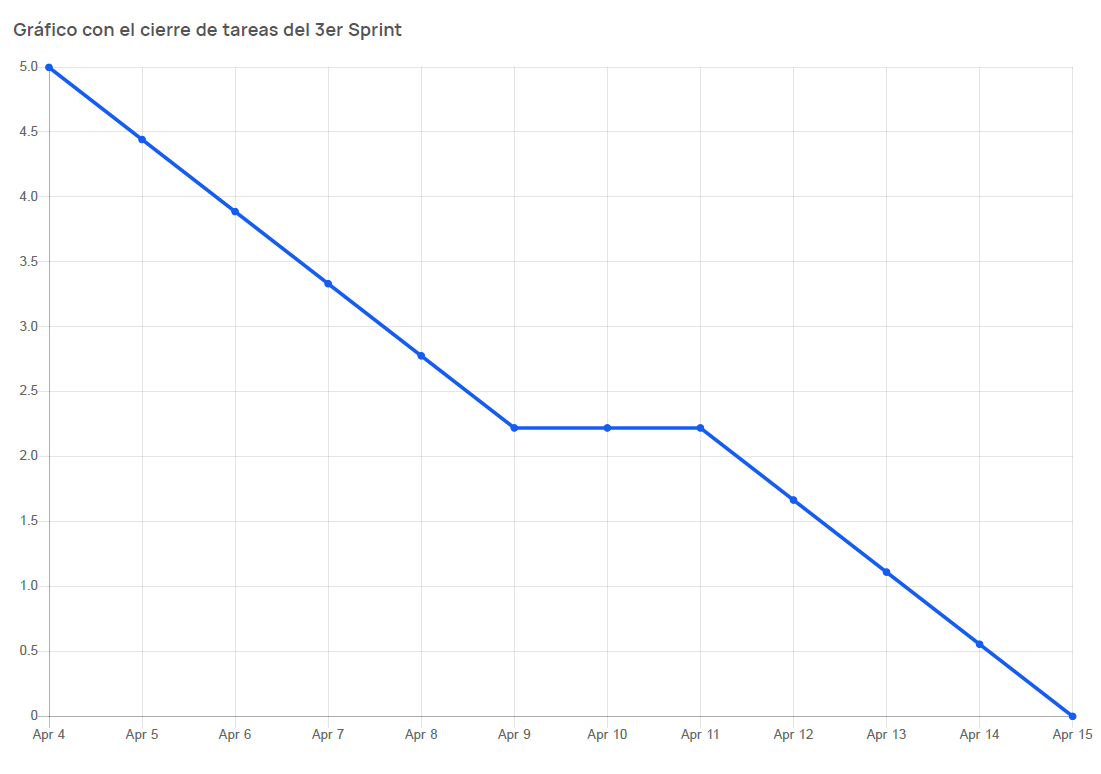
\includegraphics[width=0.6\textwidth]{img/sprint3.PNG}
\caption{Cierre de tareas del SPRINT 3}
\end{figure}
\subsection{\textbf{Sprint 4 (18/04/2022-29/04/2022)}}
El objetivo de llevar a cabo la implementación de los métodos descritos en el anterior sprint en un script, era para poder dotar a la pinza de funciones reales como si fuera el robot. De esta manera, en este sprint el objetivo buscado era fusionar tanto la replicación virtual del robot con la tecnología de los guantes y las gafas desarrollada en el segundo sprint.

Las tareas seleccionadas para este sprint fueron:
\begin{itemize}
    \item Mejorar la automatización de la apertura y cierre de la pinza.
    \item Creación de nueva escena donde serán apreciados los resultados.
    \item Adaptación de la escena de la pinza a esta nueva mediante realidad virtual\cite{VR}
    \item Mostrar virtualmente la representación de las manos en la escena.
    \item Diseñar idea que permita conectar los guantes y la pinza.
    \item Desarrollo del script conector que \begin{enumerate}
        \item Desplace la pinza a una posición cercana de las manos a una velocidad dada.
        \item Abra o cierre la pinza simulada en función de la apertura de nuestro dedo índice y pulgar, dada una velocidad.
    \end{enumerate}
    \item Fusionar todos los puntos en la escena.
    \item Ejecutar pruebas de desplazamiento y apertura para comprobar el correcto funcionamiento.
\end{itemize}

\begin{figure}[h]
\centering
\label{Cierre de tareas del SPRINT 4}
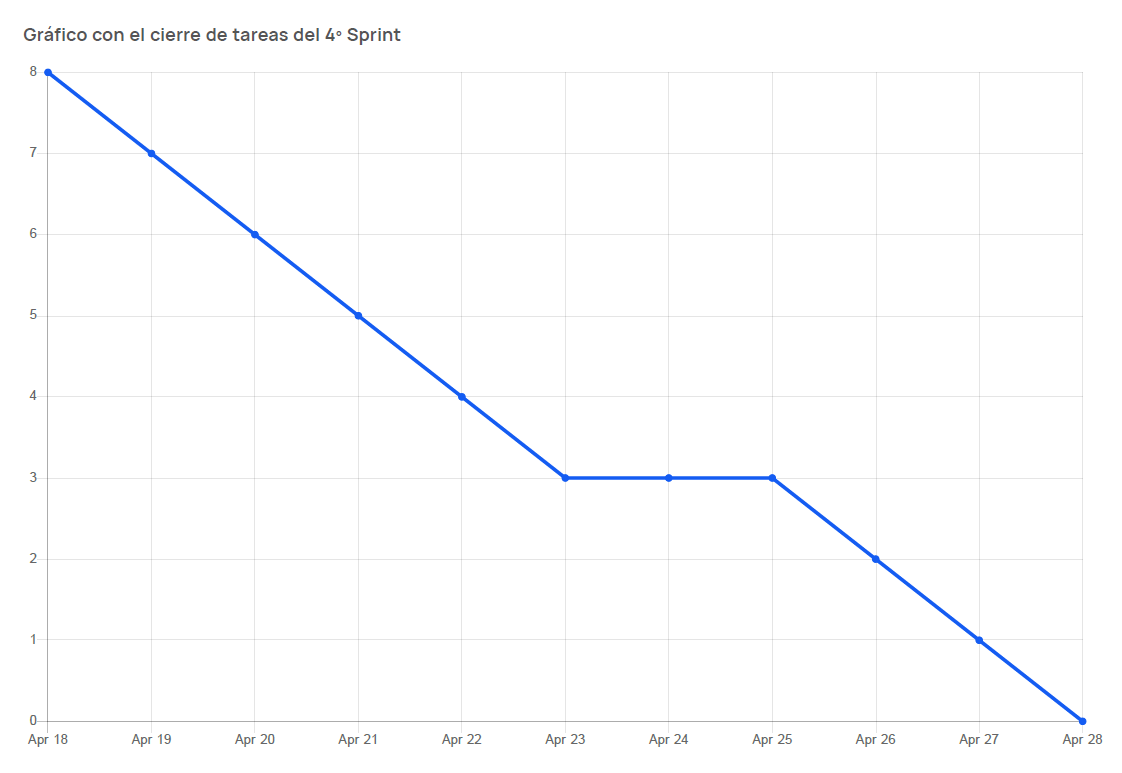
\includegraphics[width=0.6\textwidth]{img/sprint4.PNG}
\caption{Cierre de tareas del SPRINT 4}
\end{figure}
\subsection{\textbf{Sprint 5 (02/05/2022-13/05/2022)}}
Este sprint estaba pensado para comenzar a trabajar con el robot real, ya buscando resultados que den valor a lo realizado durante el proyecto. De esta manera tanto este como el siguiente sprint se antojan como unos de los más complicados, ya que nunca había trabajado con robots previamente a este proyecto.

Los objetivos marcados para cumplir este sprint vienen dados por la consecución de las siguientes tareas:
\begin{itemize}
    \item Investigación y recopilación de información sobre el brazo robótico Kinova
    \item Estudio breve a modo de introducción de ROS \cite{ROS}
    \item Establecer conexión correcta con el robot.
    \item Acceder al robot y a ROS para buscar la lista de topics(funciones) disponibles.
    \item Ejecución de pruebas con el brazo robótico desde otro proyecto.
    \item Parametrización de valores y datos necesarios.
    \item Desarrollo de una nueva escena de conexión con ROS y el robot desde Unity.
    \item Desarrollar un script que permita desplazar la pinza del robot en el espacio.
\end{itemize}

A la correcta consecución de las tareas de este sprint comenzamos a ver poco a poco cual sería el funcionamiento finalmente del robot. 


\begin{figure}[h]
\centering
\label{Cierre de tareas del SPRINT 5}
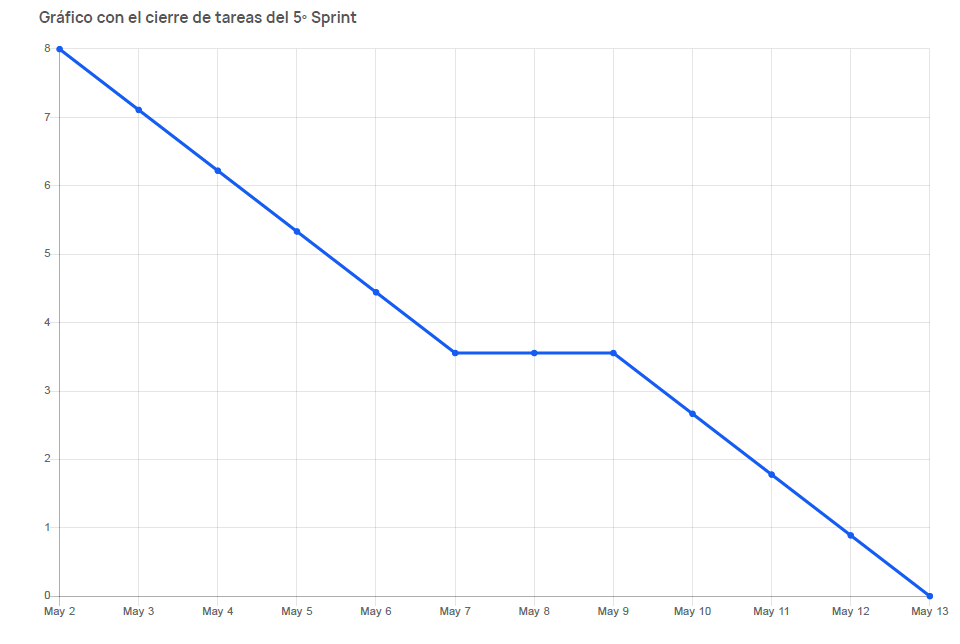
\includegraphics[width=0.6\textwidth]{img/sprint5.PNG}
\caption{Cierre de tareas del SPRINT 5}
\end{figure}
\subsection{\textbf{Sprint 6 (16/05/2022-27/05/2022)}}
Llegados al último sprint dispuesto para el proyecto, nos encontramos muy cerca de los resultados finales deseados. Por ello para este final sprint nos encargaremos de pulir algunos problemas y finalmente dejar perfilada la resolución del proyecto. En la consecución de este sprint encontraremos también la resolución positiva de los objetivos principales de proyecto marcados.

Aquí al acabar este sprint quedarían fusionadas todas las partes y tecnologías tanto vistas, como utilizadas dando lugar al resultado final.

Para finalizar el proyecto de una manera positiva y que se asemeje a lo trazado al comenzar el proyecto deberíamos cumplir las siguientes tareas:
\begin{itemize}
    \item Desarrollo de script que linkee nuestra mano con la pinza del robot y el desplazamiento en el espacio.
    \item Implementación y sincronización de rotación de la pinza con rotación de la mano.
    \item Diseño y desarrollo de un script que gestione la apertura y cierre de la pinza del robot.
    \item Limitar y gestionar valores relativos a la posición para una satisfactoria experiencia del usuario.
    \item Establecer un comando para regreso a posición 'home' para el robot.
    \item Desarrollo de la escena final donde utilizar todo lo llevado a cabo en el proyecto
    \item Ejecución de pruebas de funcionamiento.
    \item Ejecución de pruebas con desplazamiento de objetos.
    \item Filmación de vídeos que muestren el funcionamiento de lo realizado.
\end{itemize}
\newpage
\begin{figure}[h]
\centering
\label{Cierre de tareas del SPRINT 6}
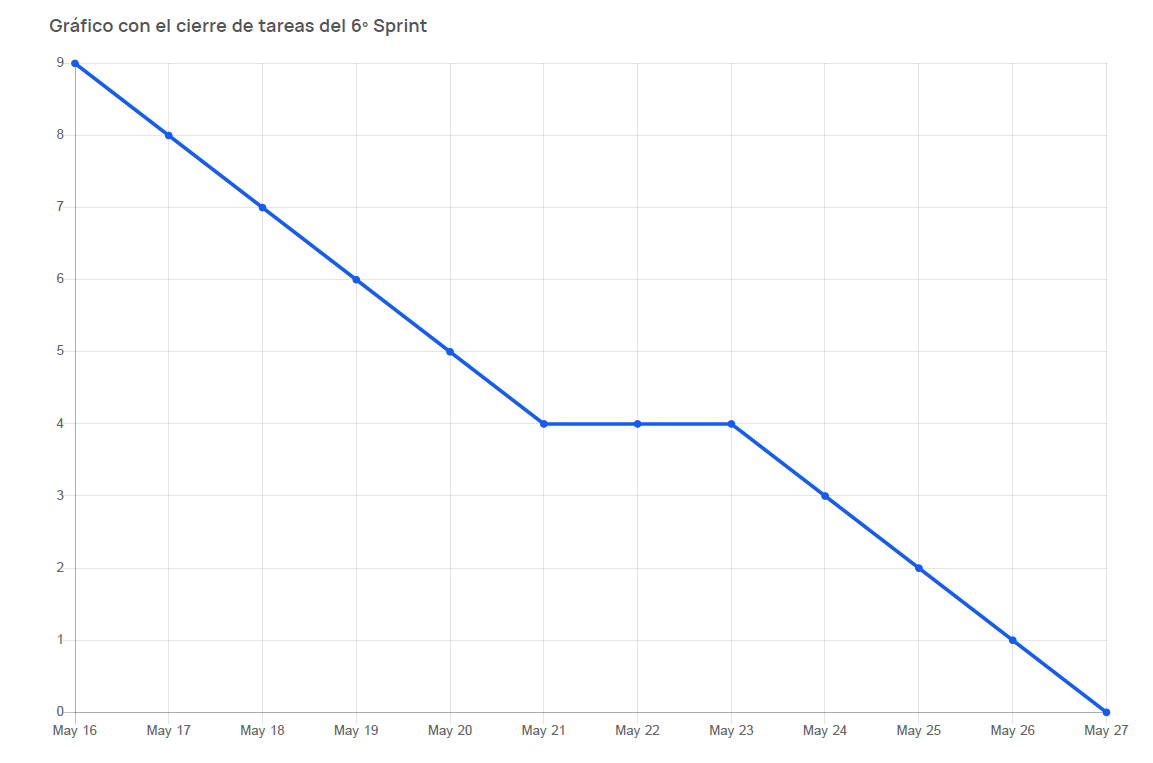
\includegraphics[width=0.6\textwidth]{img/sprint6.PNG}
\caption{Cierre de tareas del SPRINT 6}
\end{figure}
\subsection{\textbf{Final de Proyecto}}
Llegados a la última semana dentro de ITCL\cite{itcl}(30/05/2022-03/06/2022) podemos asegurar que todos los objetivos principales dispuestos han sido cumplidos correctamente, además varios de los secundarios también.

Cabe destacar que la manera de dividir las tareas y organizar el trabajo dentro del proyecto ha sido una de las cosas que ha permitido el ir consiguiendo los objetivos marcados en el tiempo marcado.

A partir de este punto el objetivo que me marco en este sprint 'personal' es el de continuar con la generación de documentación con la herramienta Overleaf, con \LaTeX que ya había ido desarrollando en paralelo con la parte de software del proyecto. De gran ayuda es para el desarrollo de esta documentación el haber ido labrando un documento a modo de diario que iba cumplimentando todas las semanas con lo hecho en esos días.

La entrega y final de esta etapa de TFG finaliza el próximo 13 de Junio de 2022 y hasta entonces el tiempo está dedicado a preparar toda la documentación, anexos y entregables.

\newpage

\section{Estudio de viabilidad}

\subsection{Viabilidad económica}
Uno de los aspectos más importantes a la hora de llevar a cabo el desarrollo de un proyecto es el de controlar los costes y derivados del mismo.

Es por ello que en este apartado dentro del anexo veremos y analizaremos estos costes. Para ello y con vista de que sea más fácil de comprender y desarrollar, dividiremos los costes totales en tres claramente diferenciados: \begin{enumerate}
    \item Coste a nivel \textbf{Hardware} 
    \item Coste a nivel \textbf{Software}
    \item Coste a nivel de \textbf{Personal}
\end{enumerate}

\newpage
\subsubsection{Coste a nivel Hardware}
Dentro de nuestro proyecto algo que juega un papel fundamental es la parte tecnológica, relacionada tanto con la tecnología de realidad virtual\cite{VR} como con la robótica\cite{Robotica} y el ordenador utilizado. Esta parte tiene un determinado coste a nivel de hardware, ya que el utilizado en el proyecto es sofisticado y especializado, que podríamos considerar por encima de lo común.

A continuación se muestra una tabla donde podemos ver tanto el nombre del producto, como el coste propio del producto y la amortización, estableciendo una amortización de cinco años y un uso de tres meses del producto.

\begin{table}[h]
    \centering
    \begin{tabular}{c| c |c}
    \hline
        Producto & Coste & Amortización \\ \hline
        SenseGlove Nova & 4499€ & 899,8€ \\
        Oculus Quest 2 & 350€ & 70€ \\
        Robot Kinova & 20.000€ & 4000€  \\
        Ordenador ITCL & 750€ & 150€ \\ \hline
        \textbf{Total} & 25.599€ & 5119,8€ \\ \hline
    \end{tabular}
    \caption{Coste a nivel Hardware}
    \label{Coste a nivel Hardware}
\end{table}

\subsubsection{Coste a nivel Software}
Otro de los aspectos que tiene vital importancia a la hora de desarrollar software es el coste específico de todos aquellos programas o licencias necesarias para llevar a cabo el desarrollo. Es por ello que a continuación vemos una tabla con el coste de software o de las licencias, considerando dos años de amortización.

\begin{table}[h]
    \centering
    \begin{tabular}{c|c|c}
    \hline
        Producto & Coste & Amortización \\ \hline
         Windows 10 Pro & 259€ & 129,5€ \\ 
         Unity Student & 0€ & 0€ \\ 
         JetBrains Rider (Student) & 0€ & 0€ \\ 
         Overleaf(\LaTeX) University & 0€ & 0€ \\ \hline
         \textbf{Total} & 259€ & 129,5€ \\ \hline
    \end{tabular}
    \caption{Coste a nivel Software}
    \label{Coste a nivel Software}
\end{table}

\subsubsection{Coste a nivel de Personal}
El último aspecto que queda por cubrir a nivel de costes es el destinado al pago del sueldo de los integrantes del personal. En este caso un único desarrollador que ha trabajado durante 300 horas dispersadas en 12 semanas, considerando un sueldo de 25000€ anuales brutos(19.880€ netos), el coste de personal sería: 

\begin{table}[h]
    \centering
    \begin{tabular}{c|c}
    \hline
        Concepto de pago & Coste  \\ \hline
       Retención por IRPF	& 333.91€ \\
       Cuota a la Seg. Social	& 147,17€ \\
       Sueldo neto mensual (12 pagas)  &  1.602,5€ \\
       Coste mensual trabajador & 2083,58€ \\ \hline
       \textbf{Coste total 12 semanas} & \textbf{6250,74€}\\ \hline
    \end{tabular}
    \caption{Costes de Personal}
    \label{Costes de Personal}
\end{table}
Estos costes se han trazado siguiendo un porcentaje de retención de IRPF del 16,03\% y una cuota de seguridad social del 28,3\%.

\subsubsection{Costes Totales}
\begin{table}[h]
    \centering
    \begin{tabular}{c|c}
       \hline Tipo Gasto & Coste  \\ \hline
         Hardware & 25.599€ \\
         Software & 129,5€ \\
         Personal & 6250,74€ \\ \hline
         \textbf{Total} & \textbf{31.979,24€} \\ \hline
    \end{tabular}
    \caption{Costes Totales}
    \label{Costes Totales}
\end{table}




\apendice{Especificación de Requisitos}

\section{Introducción}
A lo largo de este apartado veremos documentadas las posibilidades funcionales de lo desarrollado en el proyecto, centrándonos en el software final. Se especificarán cuáles eran los objetivos minimos requeridos para considerar de un buen resultado el desarrollo del proyecto, veremos tanto los requisitos funcionales como no funcionales de la aplicación
\section{Objetivos generales}
El objetivo general dentro de este proyecto a nivel de desarrollo, era el de llevar a cabo una aplicación que nos habilite a conseguir los siguientes puntos:
\begin{itemize}
    \item Establecer conexión inalámbrica entre el robot y el ordenador.
    \item Conectar el dispositivo Oculus Quest 2 a Unity\cite{Unity}
    \item Conectar los guantes Nova al ordenador y a Unity.
    \item Recoger datos relevantes de seguimiento y posicionamiento de los controladores Oculus.
    \item Recoger datos relevantes de los sensores de los guantes Nova.
    \item Representar en las tres dimensiones del espacio virtualmente nuestra mano.
    \item Desplazar la pinza del robot en las tres dimensiones del espacio siguiendo el movimiento de nuestra mano.
    \item Abrir y cerrar la pinza con un gesto de nuestra mano.
\end{itemize}
\section{Catalogo de requisitos}
Aquí veremos el catálogo de requisitos de nuestro software dividiendo en los siguientes dos:
\subsection{Requisitos Funcionales}
\begin{itemize}
    \item RF.1 Conexión entre el robot ROS\cite{ROS} y el ordenador (ROSInitializer)
    \begin{enumerate}
        \item RF.1.1 Introducir el número de IP asociada al robot.
        \item RF.1.2 Introducir el número de puerto.
        \item RF.1.3 Botón de play.
    \end{enumerate}
    \item RF.2 Recogida de datos importantes con actualización constante.
    \begin{enumerate}
        \item RF.2.1 Calibración Nova
        \item RF.2.2 Recibir datos de posición de Oculus Quest 2.
        \item RF.2.3 Recibir datos de rotación de Oculus Quest 2.
        \item RF.2.4 Recibir datos de sensores de Nova.
    \end{enumerate}
    \item RF.3 Adaptación y Aplicación de datos con actualización constante.
    \begin{enumerate}
        \item RF.3.1 Linkeo de manos con Nova en la escena.
        \item RF.3.2 Creación de mensaje de posición predeterminada(casa).
        \item RF.3.3 Creación de mensajes ROS de posición y rotación.
        \item RF.3.4 Creación de mensajes ROS de apertura de la pinza.
    \end{enumerate}
    \item RF.4 Envío de mensajes ROS al robot.
    \begin{enumerate}
        \item RF.4.1 Envío de mensaje de posición y rotación.
        \item RF.4.2 Envío de mensaje de apertura.
    \end{enumerate}
    \item RF.5 Finalizar ejecución.
    \begin{itemize}
        \item RF.5.1 Botón de finalizar conexión.
    \end{itemize}
\end{itemize}

\subsection{Requisitos No Funcionales}
A continuación veremos los requisitos  no funcionales de lo desarrollado, que se refieren a todos aquellos requisitos que describen características de funcionamiento y no las tareas que realiza o la información que guarda.


\textbf{RNF.1 - Eficiencia:} El uso del software desarrollado tiene que ser eficiente, que no provoque errores y se ejecute cumpliendo con los requisitos funcionales en tiempos lógicos(sin desarrollar grandes delays).

 \textbf{RNF.2 - Escalabilidad:} Este proyecto sirve como cimiento o base de uno de mayores proporciones, por lo que nuestro software tiene que poder ser escalable. Ya que gracias a él se podrán ver otro tipo de softwares.

\textbf{RNF.3 - Rendimiento:} El resultado de este proyecto necesita de un alto rendimiento a la hora de ejecutarlo ya que de no ser así, la experiencia del usuario se vería afectada y el software perdería valor.

 \textbf{RNF.4 - Portabilidad:} Es un requisito indispensable de este proyecto, ya que cumpliendo con ello se podrá realizar una fácil implementación junto a otros tipos de robot o de dispositivos.

\newpage

\section{Especificación de requisitos}
\begin{table}[h]
    \centering
    \begin{tabular}{| m{3cm} | m{8cm} |}
    \hline
         \multicolumn{2}{|c|}{\textbf{1. Conexión entre el robot ROS y el ordenador.}}                \\ \hline
        Requisito & 1.1 - Introducir el número de IP asociada al robot.  \\ \hline
       Autor  &  Víctor de la Iglesia García \\ \hline
        Versión & 1.0 \\ \hline
        Accion/es & Se introduce el número de IP asociado. \\ \hline
         Descripción & El usuario de esta aplicación debe introducir el número de IP asociada al robot. \\ \hline
        Precondición & Hallar el número de dirección IP. \\ \hline
        Postcondiciones & A la espera del número de puerto. \\ \hline
        Excepciones & Ninguna. \\ \hline
    \end{tabular}
    \caption{1.1 Introducir el número de IP asociada al robot.}
    \label{1.1 Introducir el número de IP asociada al robot.}
\end{table}

\begin{table}[h]
    \centering
    \begin{tabular}{| m{3cm} | m{8cm} |}
    \hline
        Requisito & 1.2 - Introducir el número de puerto.  \\ \hline
       Autor  &  Víctor de la Iglesia García \\ \hline
        Versión & 1.0 \\ \hline
        Accion/es & Se introduce el número de puerto. \\ \hline
         Descripción & El usuario de esta aplicación debe introducir el número de puerto asociada al robot. \\ \hline
        Precondición & Hallar el número de puerto. \\ \hline
        Postcondiciones & Ninguna. \\ \hline
        Excepciones & Ninguna. \\ \hline
    \end{tabular}
    \caption{1.2 - Introducir el número de puerto.}
    \label{1.2 - Introducir el número de puerto.}
\end{table}

\begin{table}[h]
    \centering
    \begin{tabular}{| m{3cm} | m{8cm} |}
    \hline
        Requisito & 1.3 - Botón de play.  \\ \hline
       Autor  &  Víctor de la Iglesia García \\ \hline
        Versión & 1.0 \\ \hline
        Accion/es & Se pulsa el botón de play.. \\ \hline
         Descripción & El usuario de esta aplicación debe pulsar el botón de play para ejecutar. \\ \hline
        Precondición & Introducir IP y número de puerto. \\ \hline
        Postcondiciones & Ninguna. \\ \hline
        Excepciones & Ninguna. \\ \hline
    \end{tabular}
    \caption{1.3 - Botón de play.}
    \label{1.3 - Botón de play.}
\end{table}

\newpage

\begin{table}[h]
    \centering
    \begin{tabular}{| m{3cm} | m{8cm} |}
    \hline
     \multicolumn{2}{|c|}{\textbf{2. Recogida de datos importantes con actualización constante.}}                \\ \hline 
        Requisito & 2.1 - Calibración Nova  \\ \hline
       Autor  &  Víctor de la Iglesia García \\ \hline
        Versión & 1.0 \\ \hline
        Accion/es & Se calibra el guante háptico Nova. \\ \hline
         Descripción & Al comenzar la ejecución se realiza una calibración de los guantes Nova. \\ \hline
        Precondición & Ejecución y tener colocado el guante. \\ \hline
        Postcondiciones & Ninguna. \\ \hline
        Excepciones & Ninguna. \\ \hline
    \end{tabular}
    \caption{2.1 - Calibración Nova}
    \label{2.1 - Calibración Nova}
\end{table}

\begin{table}[h]
    \centering
    \begin{tabular}{| m{3cm} | m{8.7cm} |}
    \hline
        Requisito & 2.2 Recibir datos de posición de Oculus Quest 2\\ \hline
       Autor  &  Víctor de la Iglesia García \\ \hline
        Versión & 1.0 \\ \hline
        Accion/es & Se recogen los datos de posición de Oculus Quest 2. \\ \hline
         Descripción & Se recogen los datos referidos a la posición de los controladores de Oculus, para poder representar correctamente en el espacio nuestras manos. \\ \hline
        Precondición & Tener las gafas cerca y estar dentro de la zona de juego de Oculus. \\ \hline
        Postcondiciones & Aplicar los datos. \\ \hline
        Excepciones & Ninguna. \\ \hline
    \end{tabular}
    \caption{2.2 Recibir datos de posición de Oculus Quest 2}
    \label{2.2 Recibir datos de posición de Oculus Quest 2}
\end{table}

\begin{table}[h]
    \centering
    \begin{tabular}{| m{3cm} | m{8.7cm} |}
    \hline
        Requisito & 2.3 Recibir datos de rotación de Oculus Quest 2\\ \hline
       Autor  &  Víctor de la Iglesia García \\ \hline
        Versión & 1.0 \\ \hline
        Accion/es & Se recogen los datos de rotación de Oculus Quest 2. \\ \hline
         Descripción & Se recogen los datos referidos a la rotación de los controladores de Oculus, para poder representar correctamente en el espacio nuestras manos. \\ \hline
        Precondición & Tener las gafas cerca y estar dentro de la zona de juego de Oculus. \\ \hline
        Postcondiciones & Aplicar los datos. \\ \hline
        Excepciones & Ninguna. \\ \hline
    \end{tabular}
    \caption{2.3 Recibir datos de rotación de Oculus Quest 2}
    \label{2.3 Recibir datos de rotación de Oculus Quest 2}
\end{table}

\newpage

\begin{table}[h]
    \centering
    \begin{tabular}{| m{3cm} | m{8cm} |}
    \hline
        Requisito & 2.4 Recibir datos de sensores de Nova\\ \hline
       Autor  &  Víctor de la Iglesia García \\ \hline
        Versión & 1.0 \\ \hline
        Accion/es & Se recogen los datos de los sensores de Nova \\ \hline
         Descripción & Se recogen los datos necesarios de los sensores de los guantes hápticos Nova. Datos de flexión de los dedos. \\ \hline
        Precondición & Tener los guantes puestos y calibrados. \\ \hline
        Postcondiciones & Aplicar los datos. \\ \hline
        Excepciones & Ninguna. \\ \hline
    \end{tabular}
    \caption{2.4 Recibir datos de sensores de Nova}
    \label{2.4 Recibir datos de sensores de Nova}
\end{table}


\begin{table}[h]
    \centering
    \begin{tabular}{| m{3cm} | m{8cm} |}
    \hline
           \multicolumn{2}{|c|}{\textbf{3. Adaptación y Aplicación de datos con actualización constante}}                \\ \hline 
        Requisito & 3.1 Linkeo de manos con Nova en la escena\\ \hline
       Autor  &  Víctor de la Iglesia García \\ \hline
        Versión & 1.0 \\ \hline
        Accion/es & Se representan nuestras manos con los datos de los sensores\\ \hline
         Descripción & Se representan nuestras manos en el espacio dentro de la escena de Unity, de manera realista y con actualización constante. \\ \hline
        Precondición & Tener los guantes puestos y calibrados con los controladores montados. \\ \hline
        Postcondiciones & Transmitir al robot. \\ \hline
        Excepciones & Ninguna. \\ \hline
    \end{tabular}
    \caption{3.1 Linkeo de manos con Nova en la escena}
    \label{3.1 Linkeo de manos con Nova en la escena}
\end{table}

\begin{table}[h]
    \centering
    \begin{tabular}{| m{3cm} | m{8cm} |}
    \hline
        Requisito & 3.2 Creación de mensaje de posición predeterminada(casa).\\ \hline
       Autor  &  Víctor de la Iglesia García \\ \hline
        Versión & 1.0 \\ \hline
        Accion/es & Se crea un mensaje de posición predeterminada.\\ \hline
         Descripción & Se crea un mensaje que llevará la pinza de nuestro brazo robótico al punto del espacio que hemos seleccionado como predeterminado. \\ \hline
        Precondición & Tener conexión con el robot. \\ \hline
        Postcondiciones & Envíar mensajes. \\ \hline
        Excepciones & Ninguna. \\ \hline
    \end{tabular}
    \caption{3.2 Creación de mensaje de posición predeterminada(casa).}
    \label{3.2 Creación de mensaje de posición predeterminada(casa).}
\end{table}

\begin{table}[h]
    \centering
    \begin{tabular}{| m{3cm} | m{8cm} |}
    \hline
        Requisito & 3.3 Creación de mensajes ROS de posición y rotación.\\ \hline
       Autor  &  Víctor de la Iglesia García \\ \hline
        Versión & 1.0 \\ \hline
        Accion/es & Se crean mensajes de posición y rotación para nuestro robot.\\ \hline
         Descripción & Se crean mensajes que nuestro robot interpreta y que llevará la pinza de nuestro brazo robótico al punto del espacio y con la rotación que le indiquemos con nuestro guante. \\ \hline
        Precondición & Tener conexión con el robot, los guantes puestos y las gafas conectadas para seguir nuestras manos. \\ \hline
        Postcondiciones & Envíar mensajes. \\ \hline
        Excepciones & Ninguna. \\ \hline
    \end{tabular}
    \caption{3.3 Creación de mensajes ROS de posición y rotación.}
    \label{3.3 Creación de mensajes ROS de posición y rotación.}
\end{table}

\begin{table}[h]
    \centering
    \begin{tabular}{| m{3cm} | m{8cm} |}
    \hline
        Requisito & 3.4 Creación de mensajes ROS de apertura de la pinza.\\ \hline
       Autor  &  Víctor de la Iglesia García \\ \hline
        Versión & 1.0 \\ \hline
        Accion/es & Se crean mensajes de apertura de la pinza para nuestro robot.\\ \hline
         Descripción & Se crean mensajes que nuestro robot interpreta y que abrirá o cerrará la pinza del robot según le indiquemos con nuestra mano. \\ \hline
        Precondición & Tener conexión con el robot, los guantes puestos y las gafas conectadas para seguir nuestras manos. \\ \hline
        Postcondiciones & Envíar mensajes. \\ \hline
        Excepciones & Ninguna. \\ \hline
    \end{tabular}
    \caption{3.4 Creación de mensajes ROS de apertura de la pinza.}
    \label{3.4 Creación de mensajes ROS de apertura de la pinza.}
\end{table}

\begin{table}[h]
    \centering
    \begin{tabular}{| m{3cm} | m{8cm} |}
    \hline
       \multicolumn{2}{|c|}{\textbf{4. Envío de mensajes ROS al robot}}                \\ \hline 
        Requisito & 4.1 Envío de mensajes de posición y rotación\\ \hline
       Autor  &  Víctor de la Iglesia García \\ \hline
        Versión & 1.0 \\ \hline
        Accion/es & Se envían los mensajes de posición y rotación de la pinza para nuestro robot.\\ \hline
         Descripción & Se envían los mensajes que nuestro robot interpretará y que colocará la pinza del robot en el espacio según le indiquemos con nuestra mano. \\ \hline
        Precondición & Creación de mensajes actualizados. \\ \hline
        Postcondiciones & Ninguna. \\ \hline
        Excepciones & Ninguna. \\ \hline
    \end{tabular}
    \caption{4.1 Envío de mensaje de posición y rotación}
    \label{4.1 Envío de mensaje de posición y rotación}
\end{table}

\begin{table}[h]
    \centering
    \begin{tabular}{| m{3cm} | m{8cm} |}
    \hline
        Requisito & 4.2 Envío de mensajes de apertura\\ \hline
       Autor  &  Víctor de la Iglesia García \\ \hline
        Versión & 1.0 \\ \hline
        Accion/es & Se envían los mensajes de apertura de la pinza para nuestro robot.\\ \hline
         Descripción & Se envían los mensajes que nuestro robot interpretará y que abrirá o cerrará la pinza del robot según le indiquemos con nuestra mano. \\ \hline
        Precondición & Creación de mensajes actualizados. \\ \hline
        Postcondiciones & Ninguna. \\ \hline
        Excepciones & Ninguna. \\ \hline
    \end{tabular}
    \caption{4.2 Envío de mensajes de apertura}
    \label{4.2 Envío de mensajes de apertura}
\end{table}

\begin{table}[h]
    \centering
    \begin{tabular}{| m{3cm} | m{8cm} |}
    \hline
       \multicolumn{2}{|c|}{\textbf{5. Finalizar ejecución}}                \\ \hline 
        Requisito & 5.1 Botón de finalizar conexión.\\ \hline
       Autor  &  Víctor de la Iglesia García \\ \hline
        Versión & 1.0 \\ \hline
        Accion/es & Se pulsa el botón que finaliza la ejecución. \\ \hline
        Descripción & Se finalizan todos los procesos y se termina la conexión con el robot. \\ \hline
        Precondición & Ninguno. \\ \hline
        Postcondiciones & Ninguna. \\ \hline
        Excepciones & Ninguna. \\ \hline
    \end{tabular}
    \caption{5.1 Botón de finalizar conexión.}
    \label{5.1 Botón de finalizar conexión.}
\end{table}









\apendice{Especificación de diseño}

\section{Introducción}
A lo largo de este punto veremos la especificación de diseño, donde veremos en profundidad que tipo de datos maneja y trata nuestra aplicación.

\section{Diseño de datos}
Aquí veremos qué datos se recogen, se generan y se aplican en nuestro software.

Los tipos datos de entrada que son utilizados en esta aplicación podríamos dividirlos en dos debido a su naturaleza, teniendo en cuenta que ambos son recogidos por los dispositivos de realidad virtual \cite{VR} de los que disponemos.

\subsection{Datos de Entrada}
    \begin{itemize}
        \item \textbf{Coordenadas de posición:} El tipo de datos más importante dentro de nuestro software es aquel referente a las coordenadas de posición que recoge Unity a través de nuestros controladores y las gafas de Oculus. Son coordenadas englobadas en un tipo de Unity que es un vector que tiene tres valores, ya que representan las tres dimensiones del espacio X Y Z.
        Como hemos visto previamente en este documento y en la memoria, este tipo de datos es el que nos da la posibilidad de representar correctamente nuestras manos en el espacio tridimensional, además de ser indispensable para poder enviar las instrucciones de posición necesarias a nuestro robot.
        
        Estos datos se recogen gracias a las gafas que a través de sus cámaras y sensores permite conocer en que punto de la zona establecida para usar Oculus se encuentran los controladores.
        
        Estos datos una vez recogidos, se procesan de manera que cumplan con el estándar establecido por mi previamente en búsqueda de una experiencia del usuario correcta. 
        
        \item \textbf{Datos de flexión y aducción}: Este tipo de datos es el que nos dará la posibilidad de aplicar un cierre o apertura determinado a nuestra pinza robótica. Se recogen directamente de los sensores dispuestos en el guante háptico y reflejan en un vector de tres partes los valores de pronación/supinación, flexión/extensión y adducción/abudcción de los dedos. 
        
        Los que utilizamos principalmente son los de flexión/extensión, ya que gracias a ellos podemos definir correctamente un comportamiento para la aplicación asociado a flexionar índice y pulgar simulando la pinza.
        
        Estos datos se recogen garcias al script \textit{GettingData}  y se pasan en forma de mensajes(instrucciones) para la pinza y así abrir o cerrar la pinza.
  \end{itemize}
  
\subsection{Datos Generados}
        Los datos que se generan en esta aplicación son mensajes ROS que se publican en los topics determinados, para hacer al robot cumplir con la tarea determinada. En este caso se generan dos tipos de mensajes específicos, unos referentes a la posición y rotación de la pinza y otros en relación con la apertura/cierre de la misma. 
        
        Estos mensajes se generan de manera constante ya que sus funciones se ejecutan constántemente mientras la aplicación esté funcionando. De esta manera conseguimos un resultado óptimo sin demasiado delay.

\section{Diseño arquitectónico}
En cuanto a la arquitectura dentro de este proyecto cabe destacar, que aunque el software final es una recopilación de objetos y técnicas utilizadas a lo largo del proyecto, hasta llegar a ese punto ha sido necesario del desarrollo de varias escenas para el aprendizaje y el análisis de cómo se gestionan o recogen los datos.

Cada una de esas escenas fue llevándose a cabo para cumplir pequeñas tareas y utilizando scripts que nos permitirían en un futuro, alcanzar el resultado que tenemos.

En el siguiente diagrama podemos ver la arquitectura del software final, donde cada una de las funciones o procedimientos que vemos están realizadas por scripts desarrollados:

\begin{figure}[h]
\centering
\label{Diagrama de la arquitectura del software final}
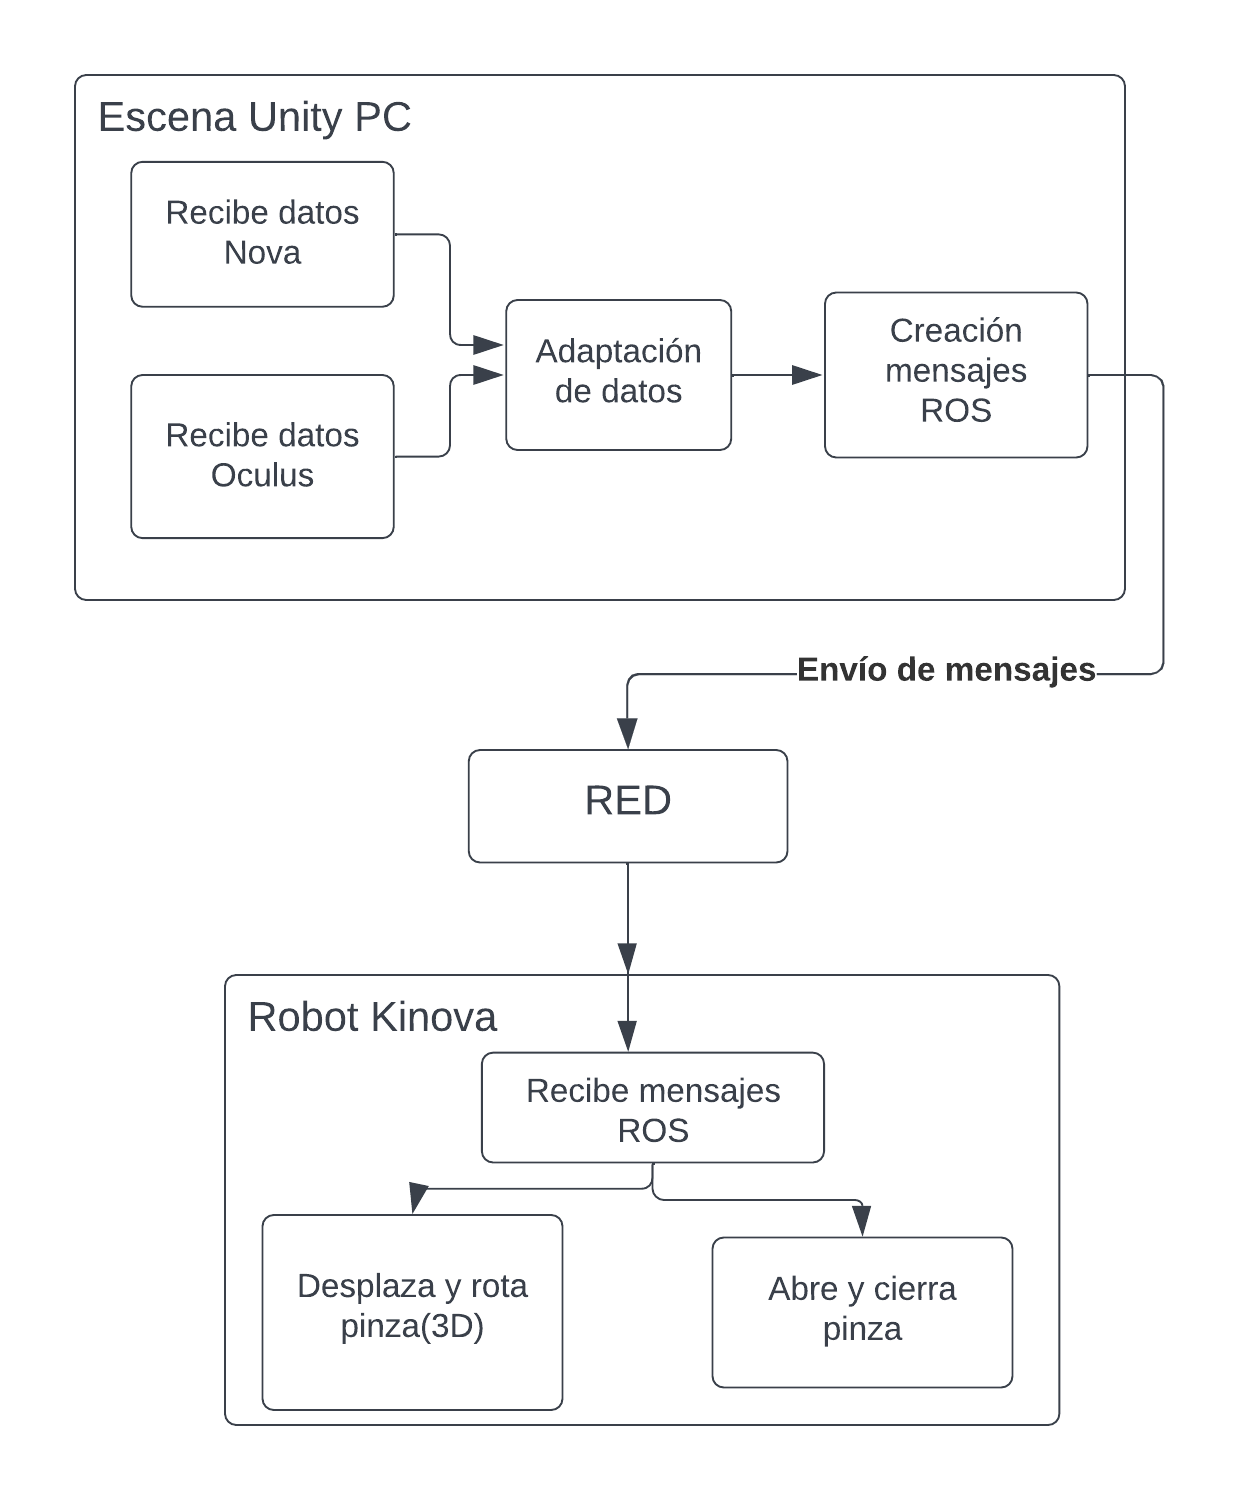
\includegraphics[width=0.9\textwidth]{img/diagrama arquitectura.png}
\caption{Diagrama de la arquitectura del software final}
\end{figure}



\apendice{Documentación técnica de programación}
\section{Introducción}
En esta parte del anexo pasaremos a ver de qué manera se halla organizado el proyecto con su estructura de directorios y archivos, también veremos todo aquello fundamental para la instalación del proyecto y poder ejecutarlo o trabajar con ello. También se verá la manera en qué se compila y se ejecuta, todo ello con documentación gráfica sobre los procesos. 

A parte de aquellos requerimientos que sean especificados a lo largo de este apéndice, también será fundamental para usarlo o trabajar con ello conocimientos específicos tanto de Unity como de C\#.

\section{Estructura de directorios}
El directorio del proyecto es el que se muestra a continuación, aunque pueda contener variaciones debido a temas de confidencialidad:
\begin{itemize}
\item \textbf{Proyecto/Assets} En esta carpeta se hayan contenidos todos los ficheros relacionados con las escenas, scripts y plugins añadidos.	
\begin{itemize}
    \item \textbf{/Assets/Art} Carpeta que contiene el arte utilizado en el proyecto.
    \item \textbf{/Assets/MyScripts} Carpeta que contiene los Scripts desarrollados para el proyecto.
    \item \textbf{/Assets/Oculus} Carpeta derivada de la descarga del plugin de Oculus para Unity.
    \item \textbf{/Assets/Prefabs} Carpeta que contienen objetos de las escenas.
    \item \textbf{/Assets/Resources} 
    \item \textbf{/Assets/RobotConnector} Carpeta que contiene Scripts para el trabajo con el robot.
    \item \textbf{/Assets/ROSBridgeLib-master} Carpeta con librerías que sirven de puente entre ROS y Unity.
    \item \textbf{/Assets/Scenes} Carpeta que contiene las escenas desarrolladas por mi en el proyecto. Es la carpeta que contiene desde los pequeños resultados que se iban consiguiendo, hasta la escena \textit{Ros} con el software final.
    \item \textbf{/Assets/SenseGlove} Carpeta que contiene las librerías para el uso de SenseGlove Nova en Unity.
    \item \textbf{/Assets/TextMesh Pro} Carpeta derivada de la instalación del plugin TextMeshPro.
    \item \textbf{/Assets/XR} Carpeta derivada de la instalación del plugin XR.
    
\end{itemize}
\item\textbf{Proyecto/Library} En esta carpeta se hayan contenidas las librerías de las que dispone Unity.
\item\textbf{Proyecto/Logs} En esta carpeta se contienen logs(registros).
\item\textbf{Proyecto/obj} 
\item\textbf{Proyecto/Packages} Carpeta que contiene datos sobre los paquetes instalados en Unity.
\item\textbf{Proyecto/ProjectSettings} Carpeta que contiene información sobre la configuración de proyecto.
\item\textbf{Proyecto/Temp} Carpeta que contiene archivos temporales.
\item\textbf{Proyecto/UserSettings} Carpeta que contiene configuración del usuario.
\end{itemize}

\newpage
\section{Manual del programador}
En esta sección prepararemos nuestro entorno de cara a poder compilar, instalar y ejecutar el proyecto en sí. Para ello veremos qué instalaciones son requeridas para el correcto trabajo, los pasos necesarios y aquellos requerimientos de PC destacados. 
En primer lugar vemos los requisitos mínimos y recomendados de Unity para ser instalado y que funcione correctamente:

\begin{figure}[h]
\centering
\label{Requisitos mínimos y recomendados Unity}
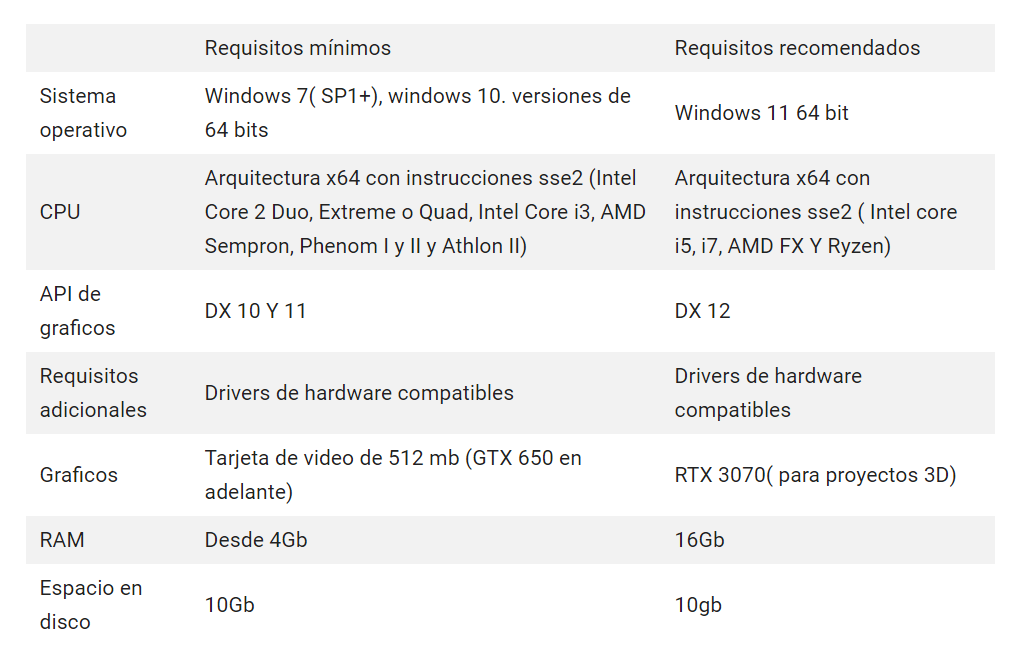
\includegraphics[width=\textwidth]{img/unity req.PNG}
\caption{Requisitos mínimos y recomendados Unity \cite{Requerimientos}}
\end{figure}

\subsubsection{Instalando Unity}
Para comenzar con la instalación es necesario acceder a su página web, donde debemos registrarnos y seleccionar el tipo de cuenta por la licencia de uso y se nos descargará el ejecutable UnityHub en su última versión (La 3.1.2 actualmente).

Deberemos de seleccionar el lugar de instalación de este programa que nos permitirá gestionar nuestros proyectos.
Después, se nos abrirá una ventana del Unity Hub donde en el apartado de Projects podremos en un futuro ver qué proyectos tenemos, vamos a la pestaña de instalaciones y veremos lo siguiente:

\newpage
\begin{figure}[h]
\centering
\label{Instalación Editor Unity 1}
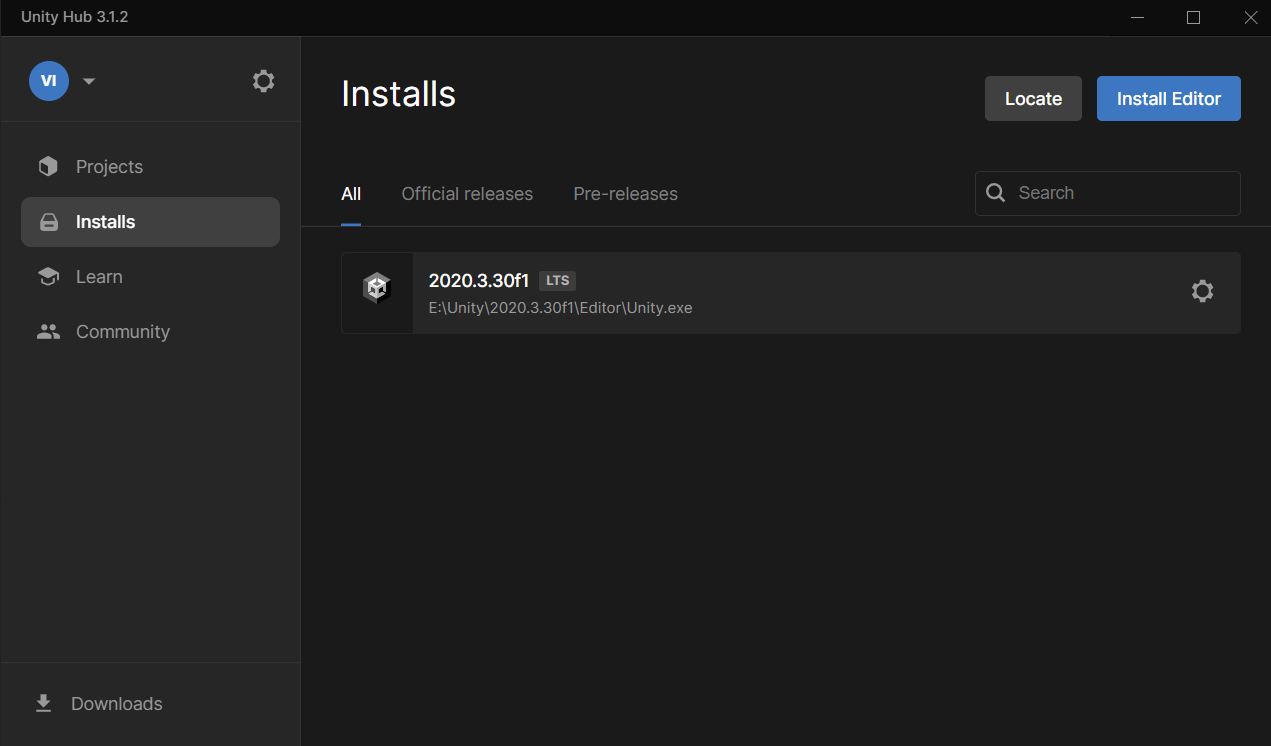
\includegraphics[width=\textwidth]{img/hub1.PNG}
\caption{Instalación Editor Unity 1 }
\end{figure}

Llegados a este punto seleccionando en instalar editor nos aparecerá la siguiente ventana que nos permitirá seleccionar la versión del editor que queramos utilizar. Recomiendo para el uso de este proyecto la versión 2020.3.30f1 ya que es con el que ha sido desarrollado y el cambio de versiones de editor puede acarrear fallos o problemas inesperados.


\begin{figure}[h]
\centering
\label{Instalación Editor Unity 2}
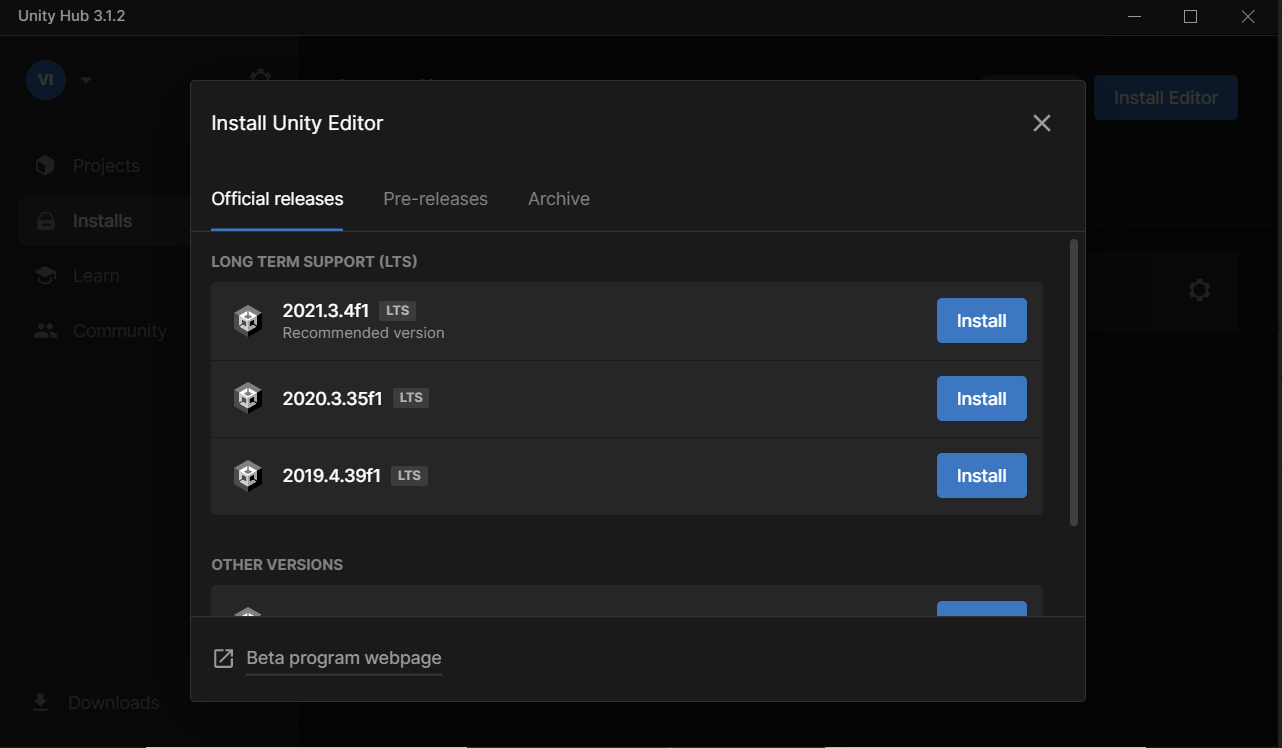
\includegraphics[width=\textwidth]{img/hub2.PNG}
\caption{Instalación Editor Unity 2}
\end{figure}


\newpage


\newpage
\subsubsection{Componentes Software}
Para poder hacer uso de nuestros dispositivos de realidad virtual necesitaremos del software especializado requerido. Por ello aquí veremos qué necesitamos instalar en nuestro ordenador.
\begin{itemize}
    \item \textbf{SenseCom}:
    Este software es el necesario de instalar para poder utilizar nuestros guantes hápticos, para ello nos dirigiremos a la página web de \textit{senseglove.com} y accederemos al apartado de developers. Desde ese apartado podremos adentrarnos en el proyecto de GitHub SenseGlove-API, el cual contiene un ejecutable que instalará este software.
    
    Se muestra a continuación una imagen del contenido de lo descargado junto a la pantalla de instalación, tras ejecutar el instalador.
    
    \begin{figure}[h]
\centering
\label{Instalación Software SenseGlove}
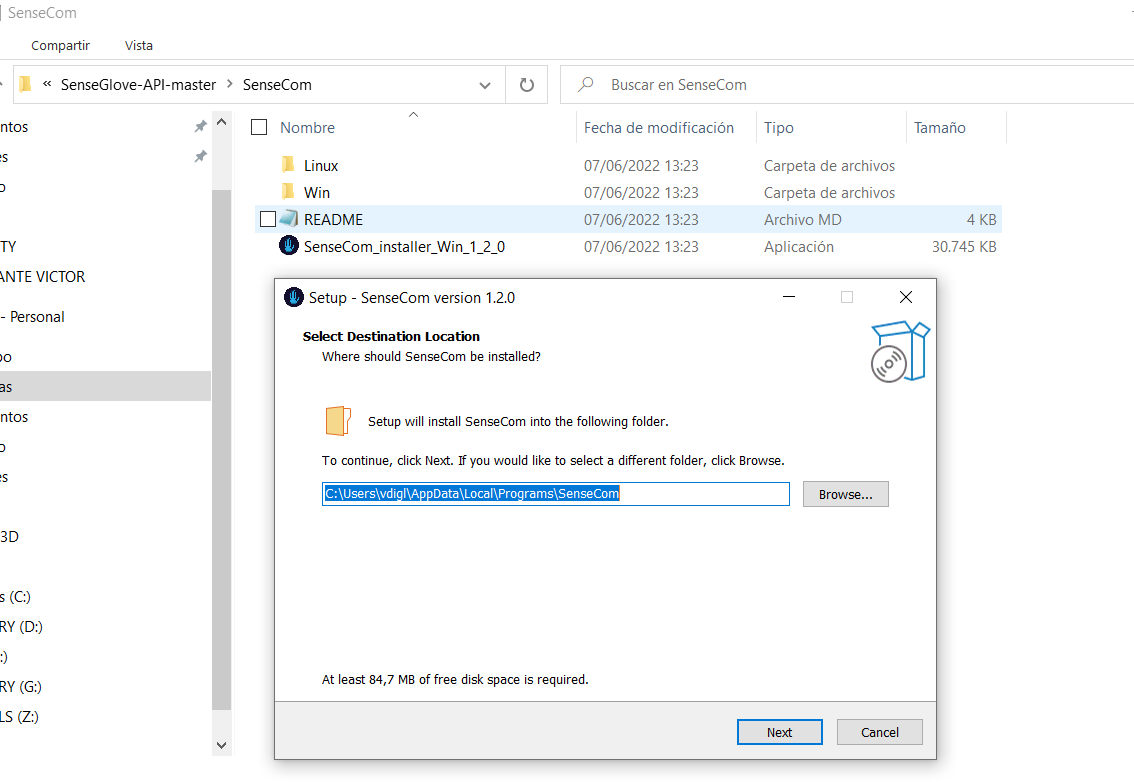
\includegraphics[width=1.1\textwidth]{img/sensecom01.PNG}
\caption{Instalación Software SenseGlove}
\end{figure}

\newpage
\item \textbf{Oculus}:
El siguiente software que debemos instalar en nuestro PC es el de Oculus\cite{Quest2} ya que sin el, no podremos conectar nuestro dispositivo Oculus Quest 2 ni sus controladores a Unity. 
Para esta instalación, accederemos a la siguiente página web => \textit{https://store.facebook.com/es/quest/setup/} y descargaremos el software.

En este punto se nos descargará un archivo \textit{OculusSetup.exe}, el cual debemos ejecutar, y tras revisar los términos y condiciones nos aparecerá la siguiente pantalla:

    \begin{figure}[h]
\centering
\label{Instalación Software Oculus}
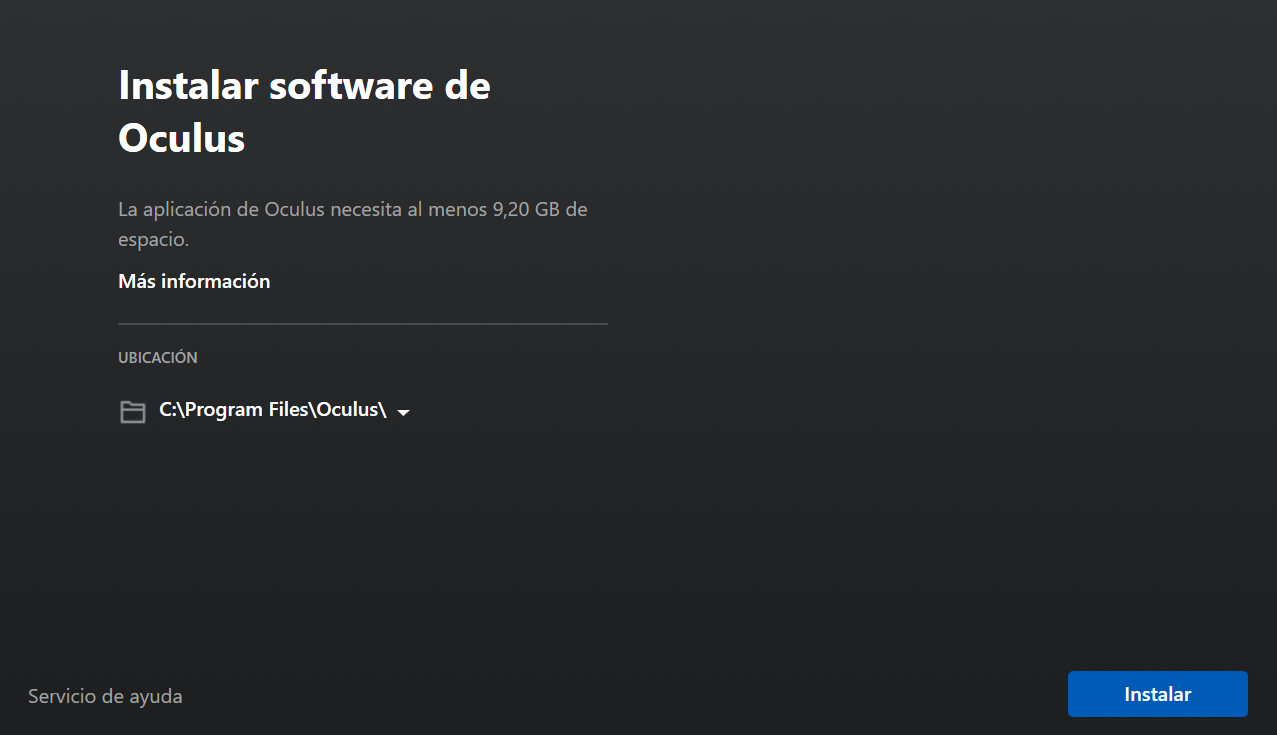
\includegraphics[width=1.1\textwidth]{img/oculus.PNG}
\caption{Instalación Software Oculus}
\end{figure}

\newpage
Tras realizar la instalación se nos requerirá de la creación de una cuenta que puede ser de \textit{Facebook} y posteriormente a todo este proceso, ya podremos configurar nuestro hardware y simplemente con tener las gafas conectadas al PC podremos usar los dispositivos desde Unity.

\item \textbf{IP Advanced Scanner}: Para descargar este software, que nos servirá de gran ayuda a la hora de preparar la conexión con nuestro robot debemos acceder a la web oficial que es la siguiente=> \textit{https://www.advanced-ip-scanner.com/es/} y realizar la descarga. Este software está configurado para poder instalarse en el ordenador o para ser ejecutado de manera única con su versión portátil.

Al correr el ejecutable se nos abre la siguiente ventana que nos permite elegir:

    \begin{figure}[h]
\centering
\label{Instalación Escáner de RED}
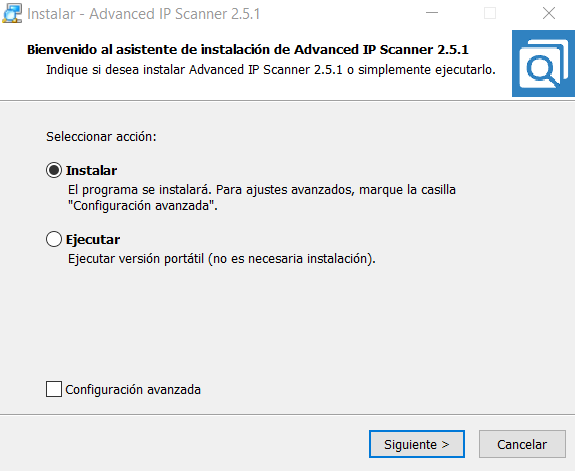
\includegraphics[width=0.9\textwidth]{img/ipad.PNG}
\caption{Instalación Escáner de RED}
\end{figure}

\newpage
Una vez aquí podemos seleccionar la opción que prefiramos, en caso de de instalar, seleccionaremos la ruta de destino de la instalación y ya tendríamos este software.

\end{itemize}


\newpage
\section{Compilación, instalación y ejecución del proyecto}
Llegados a este punto del anexo, en caso de querer utilizar el proyecto, deberíamos tener instaladas ya las aplicaciones comentadas previamente.
Ahora bien, comenzaremos con la compilación, instalación y forma de ejecutar este proyecto.

En primer lugar tendremos que comprobar tres cosas:
\begin{enumerate}
    \item Comprobar con SenseCom que tenemos conexión con los guantes, para ello debemos de tenerlos encendidos y añadidos a dispositivos bluetooth de nuestro PC. Tras esto, al abrir el software nos saldrá en pantalla que se encuentran conectados y veremos una representación de nuestras manos.
    \item Comprobar la conexión de Oculus con su software, se puede conectar vía WIFI o lo recomendado por cable, ya que la conexión es directa.
    \item Comprobar con el escáner de red instalado, la dirección IP del robot.
\end{enumerate}

Los siguientes pasos son ya relacionados con Unity.
\newpage
\subsection{Unity}
Abrimos Unity Hub y seleccionaremos el botón de \textit{Open} ya que es el que nos permite añadir proyectos a nuestro Unity. 

   \begin{figure}[h]
\centering
\label{Importar Proyecto}
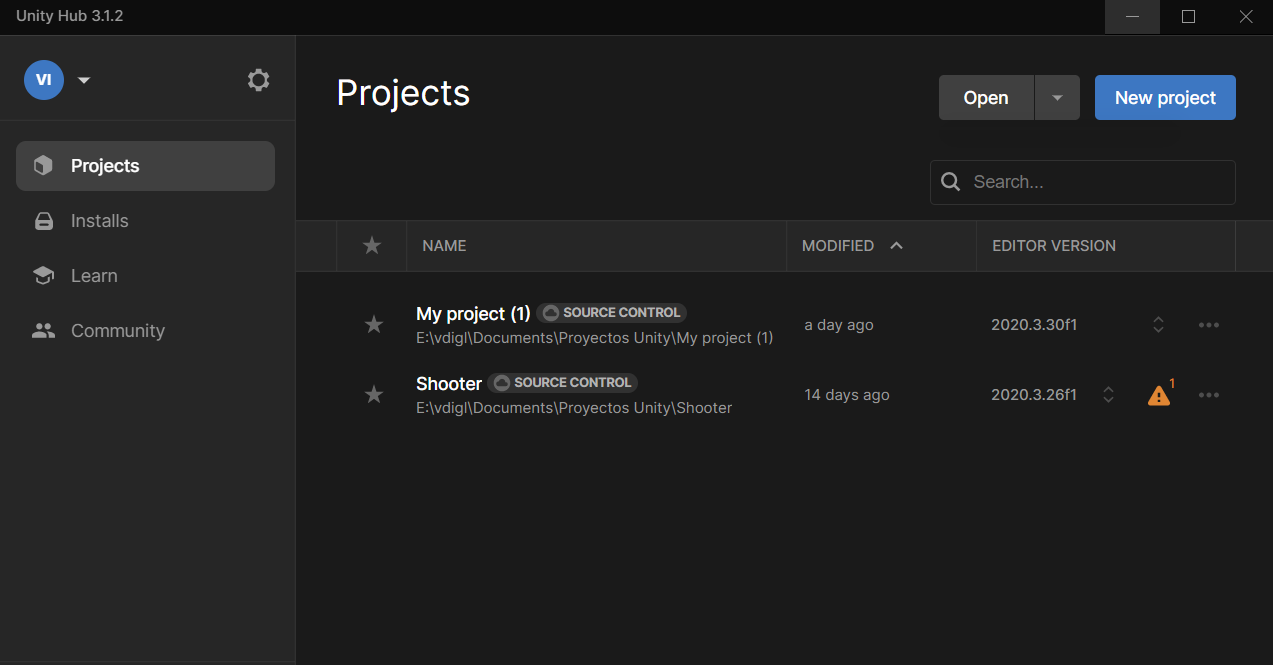
\includegraphics[width=0.9\textwidth]{img/hub3.PNG}
\caption{Importar Proyecto}
\end{figure}

Después de esto se nos abrirá la clásica ventana de nuestro explorador que nos permitirá llegar al punto donde tengamos la carpeta del proyecto, para así poder abrirlo e importarlo. Deberemos seleccionar de las versiones del editor que tengamos instaladas la que queramos utilizar para este proyecto. La recomendada por mi es la \textit{2020.3.30f1}

Recuerdo de nuevo que se recomienda siempre utilizar la versión del editor correspondiente a la de quién realizó el proyecto, ya que pueden aparecer errores o problemas de importación.

\newpage
Una vez tengamos todo importado, en la parte baja de la pantalla aparece el explorador de Unity y accedemos dentro de la carpeta \textit{Assets} a la carpeta de nombre \textit{Scenes}. Posteriormente debemos seleccionar la escena \textit{Ros} ya que es el software final del proyecto.

   \begin{figure}[h]
\centering
\label{Explorador archivos de proyecto}
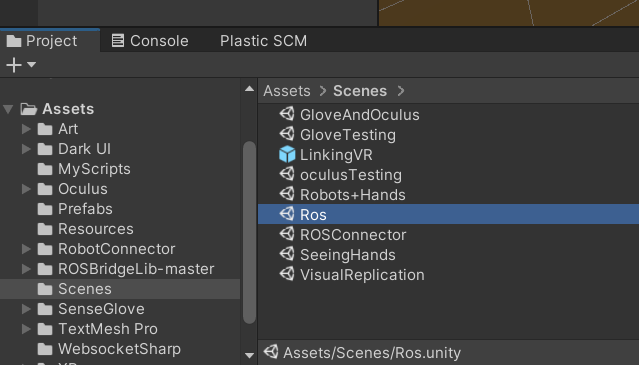
\includegraphics[width=0.9\textwidth]{img/inst1.PNG}
\caption{Explorador archivos de proyecto}
\end{figure}

Una vez abierta esta escena en la parte superior izquierda de la pantalla, nos aparecerá una jerarquía con los \textit{GameObjects}\cite{GameObjects} de nuestra escena. Debemos de seleccionar \textit{ROSInitializer} para configurar la conexión. En el lado derecho en el \textit{Inspector} nos aparecerá el siguiente cuadro: 

   \begin{figure}[h]
\centering
\label{Configuración de conexión con Robot}
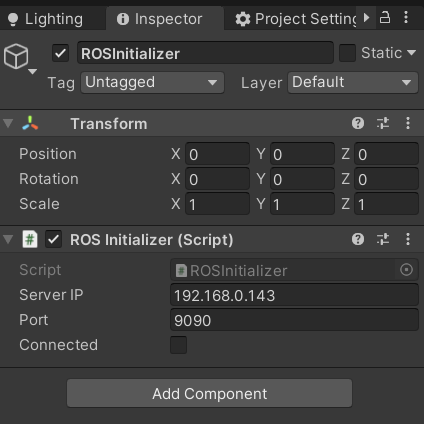
\includegraphics[width=0.45\textwidth]{img/inst2.PNG}
\caption{Configuración de conexión con Robot}
\end{figure}

En este cuadro tendremos que rellenar con el número de IP y el puerto para que a la hora de ejecutar sea capaz de conectar con el robot. El resto de los valores asociados a cada variable o componente de los \textit{GameObjects} de esta escena se deben de mantener igual.

Con todo esto ya tendremos listo el software para llevar a cabo la \textit{build} y empezar a usarlo.
Para ello en la barra superior de herramientas accedemos a => \textit{File}->\textit{Build Settings} y se nos mostrará la siguiente ventana:

   \begin{figure}[h]
\centering
\label{Realizando \textit{Build} del proyecto}
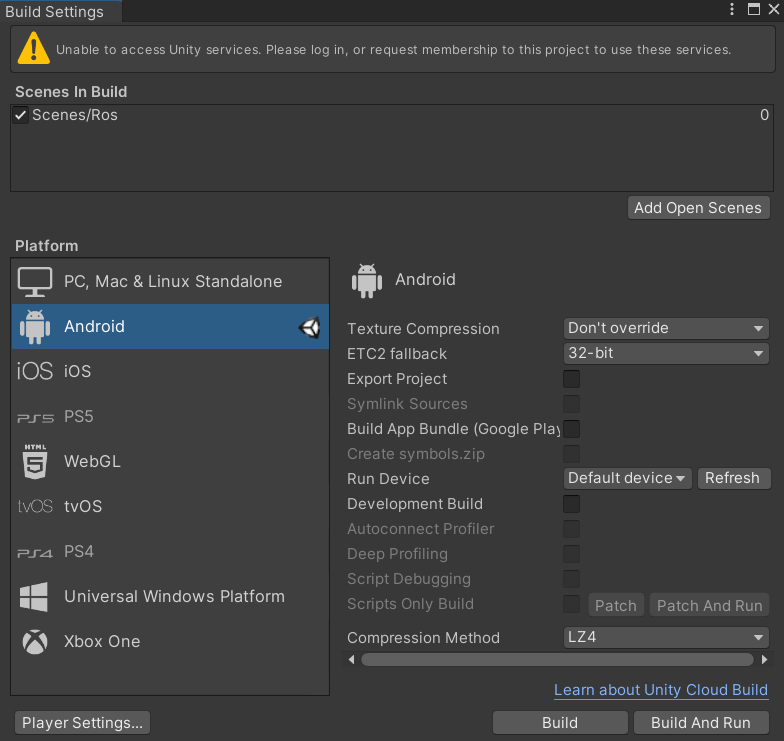
\includegraphics[width=0.8\textwidth]{img/inst3.PNG}
\caption{Realizando \textit{Build} del proyecto}
\end{figure}

En el apartado \textit{Run Device} debemos o dejarlo en dispositivo por defecto o seleccionar el dispositivo Android VR\cite{VR} (Las Oculus Quest 2 en mi caso) que queramos utilizar con Unity.
Seleccionamos \textit{Build} y se abrirá un explorador de archivos que nos permitirá alojar nuestro archivo \textit{.apk} que correremos en el dispositivo Android.

\newpage
En caso correcto, en la carpeta de destino seleccionada debemos ver el siguiente fichero .apk con el nombre seleccionado (En este caso \textit{Build1.apk}).
   \begin{figure}[h]
\centering
\label{Realizando la \textit{Build} resultante de proyecto}
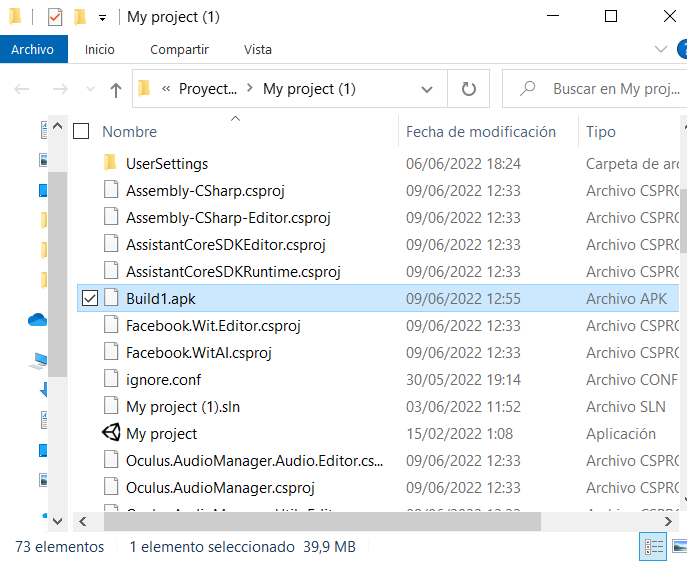
\includegraphics[width=0.8\textwidth]{img/inst4.PNG}
\caption{Realizando \textit{Build} resultante de proyecto}
\end{figure}

A partir de aquí, si tenemos conectados todos los dispositivos, solo nos quedaría pulsar el botón \textit{Run/Play} de Unity para que se ejecute el proyecto y comenzar a trabajar junto al robot y demás dispositivos.


\apendice{Documentación de usuario}
\section{Introducción}
Llegados al fin del proyecto quedaría como resultado para el usuario, una aplicación software que desde Unity con unas gafas como las Oculus Quest 2 se nos permita hacer uso de un robot mediante teleoperación. 
\section{Requisitos de usuarios}
Para poder hacer uso del software desarrollado necesitamos fundamentalmente dos dispositivos hardware relacionados con la realidad virtual distintos que son las Oculus Quest 2 y los Nova de SenseGlove, un robot con ROS como el Kinova 6DOF y un ordenador con Unity.
Para poder instalar y ejecutar correctamente Unity los requisitos son los mismos que los expuestos previamente:
\begin{figure}[h]
\centering
\label{Requisitos minimos y recomendados Unity}
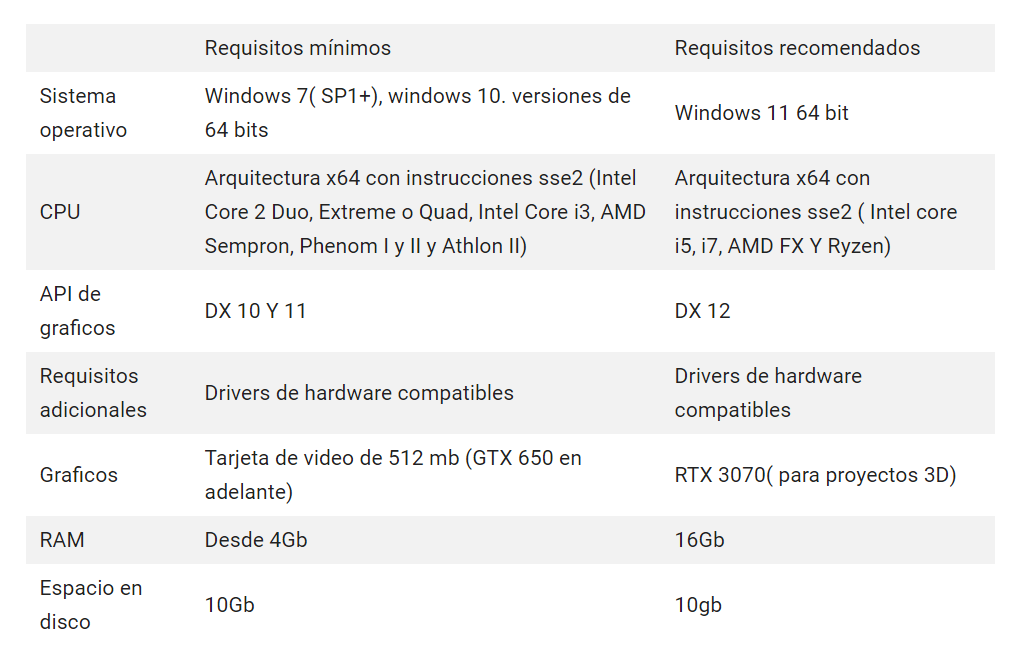
\includegraphics[width=\textwidth]{img/unity req.PNG}
\caption{Requisitos minimos y recomendados Unity}
\end{figure}

\newpage
\section{Instalación}

En cuanto a los pasos para completar la instalación del proyecto en el ordenador de un usuario, son los mismos que los expuestos en el previo apartado de \textit{Compilación, instalación y ejecución del proyecto}

\section{Manual del usuario}
Tras la debida preparación en apartados anteriores de nuestos dispositivos, una vez tengamos todos calibrados y con conexión con el PC o el robot, lo único que tenemos que hacer es ejecutar el software y aplicar sobre nuestra mano los debidos desplazamientos deseados para mover la pinza o gestualizar el cierre de la misma para controlar su apertura.




\bibliographystyle{plain}
\bibliography{bibliografiaAnexos}

\end{document}
